\documentclass[../part_2.tex]{subfiles}

\begin{document}
    \subsection{Описание данных}
    \par Первое исследование было решено провести на примерах кода на одном языке программирования, чтобы исключить из исследования возможные зависимости от разных языков.
    \par В качестве языка для эксперементов был выбран С в виду его невероятной поплуярности и представленности в разработке кода, так же синтаксис многих современных языков был основан на синтаксисе языка С.
    \par Тренировочный набор данных был собран с помощью репозитория CodeforcesYoink\cite{codeforcesyoink, cfy_text}. Он предоставляет инструмент для автоматизированного сбора примеров кода с платформы codeforces. С помощью этого инструмента можно извлекать код участников по определенным параметрам, таким как язык программирования или идентификатору задания.
    \par Были собранны данные из 104 задач. Количество тренировочных данных: 36489 примеров кода.
    \par Для оценки результата работы использованы данные из Project CodeNet\cite{puri2021codenetlargescaleaicode} от IBM. Это масштабный датасет, содержащий более 14 миллионов образцов кода на 55 языках программирования. Датасет включает разнообразные задачи, метаданные(например статус выполнения, время работы кода, потребление памяти).
    \begin{figure}[H]
        \centering
        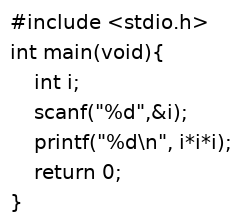
\includegraphics[width=.5\linewidth]{input_data.png}
        \caption{Пример объекта из набора данных}
    \end{figure}
    \par Из всего набора данных было отобранно 48 задач. Для каждой задачи были выбранны решения выполненные на языке программирования С с наибольшим числом решений.
\end{document}